In the following section \ref{sec:req}, an overview of the model's requirements and objective is provided, \ref{MLOPS-arch}, and the following section will give the main contributions of the work.

\section{Requirements}
\label{sec:req}
Below is an overview of the requirements for the entire NMOps architecture, which outlines the functional, non-functional, data, hardware, software, and operational requirements necessary to implement, deploy, and maintain the system.

The project focuses on processing battery cycle data of the test bench to correct the SOH estimates of a semi-empirical model, which measures the remaining capacity compared to its original state (in \%). The raw data from the test bench is ingested and processed using the Databricks Medallion Architecture, moving through the Bronze (raw), Silver (cleansed), and Gold (curated) layers to ensure data quality and readiness for analytics. This curated data is processed by the SOH semi-empirical model, resulting in the final cyclic aging. It then passes through the algorithm, which corrects it using data-driven techniques, and produces a smoothed, accurate SOH estimate. It is designed to handle individual battery datasets, with potential scalability to large fleets, and fits into an MLOps framework for continuous deployment and monitoring. 

\subsection{Functional Requirements:}
\begin{itemize}
    \item \textbf{Data Ingestion:} Read battery parameters from a JSON file containing metadata such as battery names, ambient temperature, cutoff voltage, and end-of-life capacity. Ingest processed battery cycle data for processing, outputting a dataframe with columns: cycle, Final\_cyclic\_aging, ground\_truth\_soh, and optionally others.
    \item \textbf{Data Preprocessing:} Scale Final\_cyclic\_aging to match the scale of ground\_\\truth\_soh using semi-empirical model and scaling factor.
    \item \textbf{Optimization:} Use the algorithms to optimize and correct SOH estimates from the semi-empirical model.
    \item \textbf{Stacking:} Train a linear regression model to combine final\_cycling\_aging and corrected\_soh, predicting stacked SOH that minimizes MSE against ground\\\_truth\_soh.
    \item \textbf{Smoothing:} Optimization of the parameters using Optuna, minimizing Huber Loss, and applying estimation algorithms to smooth the stacked SOH, producing smooth SOH values.
    \item \textbf{Error Estimation:} Compute error metrics: MSE\_ground\_truth, RMSE\_\\ground\_truth, MSE\_final\_cyclic, RMSE\_final\_cyclic.
    \item \textbf{Output and Visualization:} Save processed Dataframes as tables, print correction factors and error metrics, plot ground truth vs semi-empirical SOH estimates vs corrected smoothed SOH.
\end{itemize}

\subsection{Non-Functional Requirements}
These specify how the system should perform and operate.
\begin{itemize}
    \item \textbf{Performance:} Processing of battery (1000 cycles) in under 5 minutes on a standard laptop (16GB RAM, 4-core CPU). Scale to process 1000 batteries in under 24 hours with parallelization on a cloud cluster (16 vCPUs, 64GB RAM).
    \item \textbf{Accuracy:} Achieve RMSE\_ground\_truth < 1\% % for typical battery datasets, ensuring corrected SOH closely matches true SOH. Maintain robustness to outliers in final\_cycling\_aging via Huber Loss.
    \item \textbf{Scalability:} Handle datasets with up to 10,000 or 1 million cycles per battery using distributed computing or parallel processing.
    \item \textbf{Reliability:} Ensure no data loss during processing, with robust error handling for missing or corrupt data. Maintain consistent results across runs with the same input (deterministic behavior with fixed random seeds).
    \item \textbf{Maintainability:} Modular code structure to allow updates to MHE, stacking, or EKF components. Clear documentation for functions to support enhancements.
    \item \textbf{Reusability:} Provide user-friendly outputs for engineers and researchers.
    \item \textbf{Security:} Encrypt sensitive data such as battery parameters, semi-empirical model parameters, and compliance with data privacy regulations.
\end{itemize}

\subsection{Data Requirements}
A battery time series dataset, tested in the test bench, containing all relevant information such as testing conditions, nominal battery capacity, battery name, corresponding temperature, DOD, and voltage. 


\subsection{Hardware Requirements}
\begin{itemize}
    \item Laptop with 8GB RAM, 2-core CPU(e.g., Intel i5), 256GB SSD.
    \item \textbf{Cloud Cluster:} 16 vCPUs, 64GB RAM, 1TB storage.
    \item \textbf{Distributed Setup:} Spark cluster with 10 nodes (16 vCPUs, 64GB RAM each) for 10,000 batteries or 1 million cycles.
\end{itemize}

\subsection{Software Requirements}
\begin{itemize}
    \item \textbf{Programming Language:} Python 3.8+ (required for Optuna and other dependencies).
    \item \textbf{Core Libraries:} pandas, numpy, scipy, optuna, sklearn, matplotlib.
    \item \textbf{Scalability Libraries:} pyspark, tensorflow, or pytorch when extended to neural networks.
\end{itemize}

\subsection{Development Environment:}
\begin{itemize}
    \item Jupyter Notebook or Databricks environment.
    \item IDE (VS Code) for development.
    \item Git for version control.
\end{itemize}

\section{MLOps Architecture Integration Requirements}\
\label{MLOPS-arch}
To integrate the SOH estimation algorithm into an MLOps framework for correcting semi-empirical model outputs, the following requirements ensure automated, scalable, and reliable operation in production.
\begin{enumerate}
    \item Data pipeline: Kuberflow, Pandas/Spark for transformations.
    \item \textbf{Model Training Pipeline:} MLflow for logging, SageMaker for cloud training, Kuberflow for orchestration.
    \item \textbf{Model Deployment}: FastAPI for API, Docker for containerization, Kubernetes for orchestration.
    \item \textbf{Monitoring and Maintenance:} Grafana for dashboards, Prometheus for alerts.
    \item \textbf{CI/CD and Retraining:} GitHub Actions for CI, Jenkins for CD, MLflow for model versioning.
\end{enumerate}

\section{NMOps Architecture:}
The Figure \ref{fig:nmops-architecture} outlines the NMOps (Numerical Model Operations) framework for developing, deploying, and maintaining State of Health (SOH) estimation and forecasting models. The architecture leverages a combination of data engineering pipelines, semi-empirical modeling, hybrid estimation methods, and model registry principles to ensure scalable, reproducible, and production-ready solutions.

\begin{itemize}
    \item \textbf{AFM Module:} The AFM module is responsible for the synthetic collection of data from laboratory-based cell tests and vehicle field operations. This step ensures a robust and comprehensive dataset is available for downstream processing.
    \item \textbf{SOH\_c Estimation Model Data Engineering Pipeline:} The SOH\_c Estimation Model Data Engineering Pipeline module handles the preprocessing and feature engineering of the collected raw data. This includes cleaning, normalization, feature extraction, and quality assurance processes to prepare the data for the estimation model development.
    \item \textbf{Semi-Empirical (SE) Model:} The SE model is constructed using domain knowledge and empirical observations. It incorporates:
    \begin{itemize}
        \item Time Factor logic.
        \item State of Charge (SOC) Factor logic.
        \item Temperature Factor Logic.
        \item Depth of Discharge (DOD) logic.
        \item Correction Factor logic.
    \end{itemize}
    Each factor individually contributes to the overall estimation of the battery’s State of Health.
    \item \textbf{Hybrid MHE Model:} To enhance the baseline SE model, a hybrid Moving Horizon Estimation (Hybrid-MHE) framework is applied:
    \begin{itemize}
        \item \textbf{Statistical Validation:} Model performance is continuously monitored \\through statistical tests. If deviation exceeds a defined threshold, corrective action is triggered.
        \item \textbf{MHE-based Correction Factor Estimation:} A correction model is retrained dynamically based on the data-detected deviations.
        \item \textbf{Baseline Model Extraction:} Updated baseline SOH models are extracted and recorded.
        \item \textbf{Model Registry:} Models and associated regression weights and parameters are stored systematically in a model registry for traceability and reproducibility.
    \end{itemize}
    This hybrid modeling strategy enables the system to maintain high levels of accuracy while adapting to changing operating conditions.
\end{itemize}

The battery SOH estimation system has been successfully integrated into an MLOps architecture, meeting all eight requirements for a robust, scalable, and automated workflow as outlined in the section \ref{MLOPS-arch}. The implemented data pipeline ingests and preprocesses battery data seamlessly, the training pipeline optimizes and logs models efficiently, and the deployment system serves real-time and batch predictions with high availability. Comprehensive monitoring, CI/CD, security, and retraining ensure continuous accuracy and compliance, while a skilled team and cloud infrastructure support scalability to thousands of batteries. This MLOps integration transforms the algorithm into a production-ready solution, correcting semi-empirical SOH estimates for critical applications like EV fleet management.
\begin{figure}
    \centering
    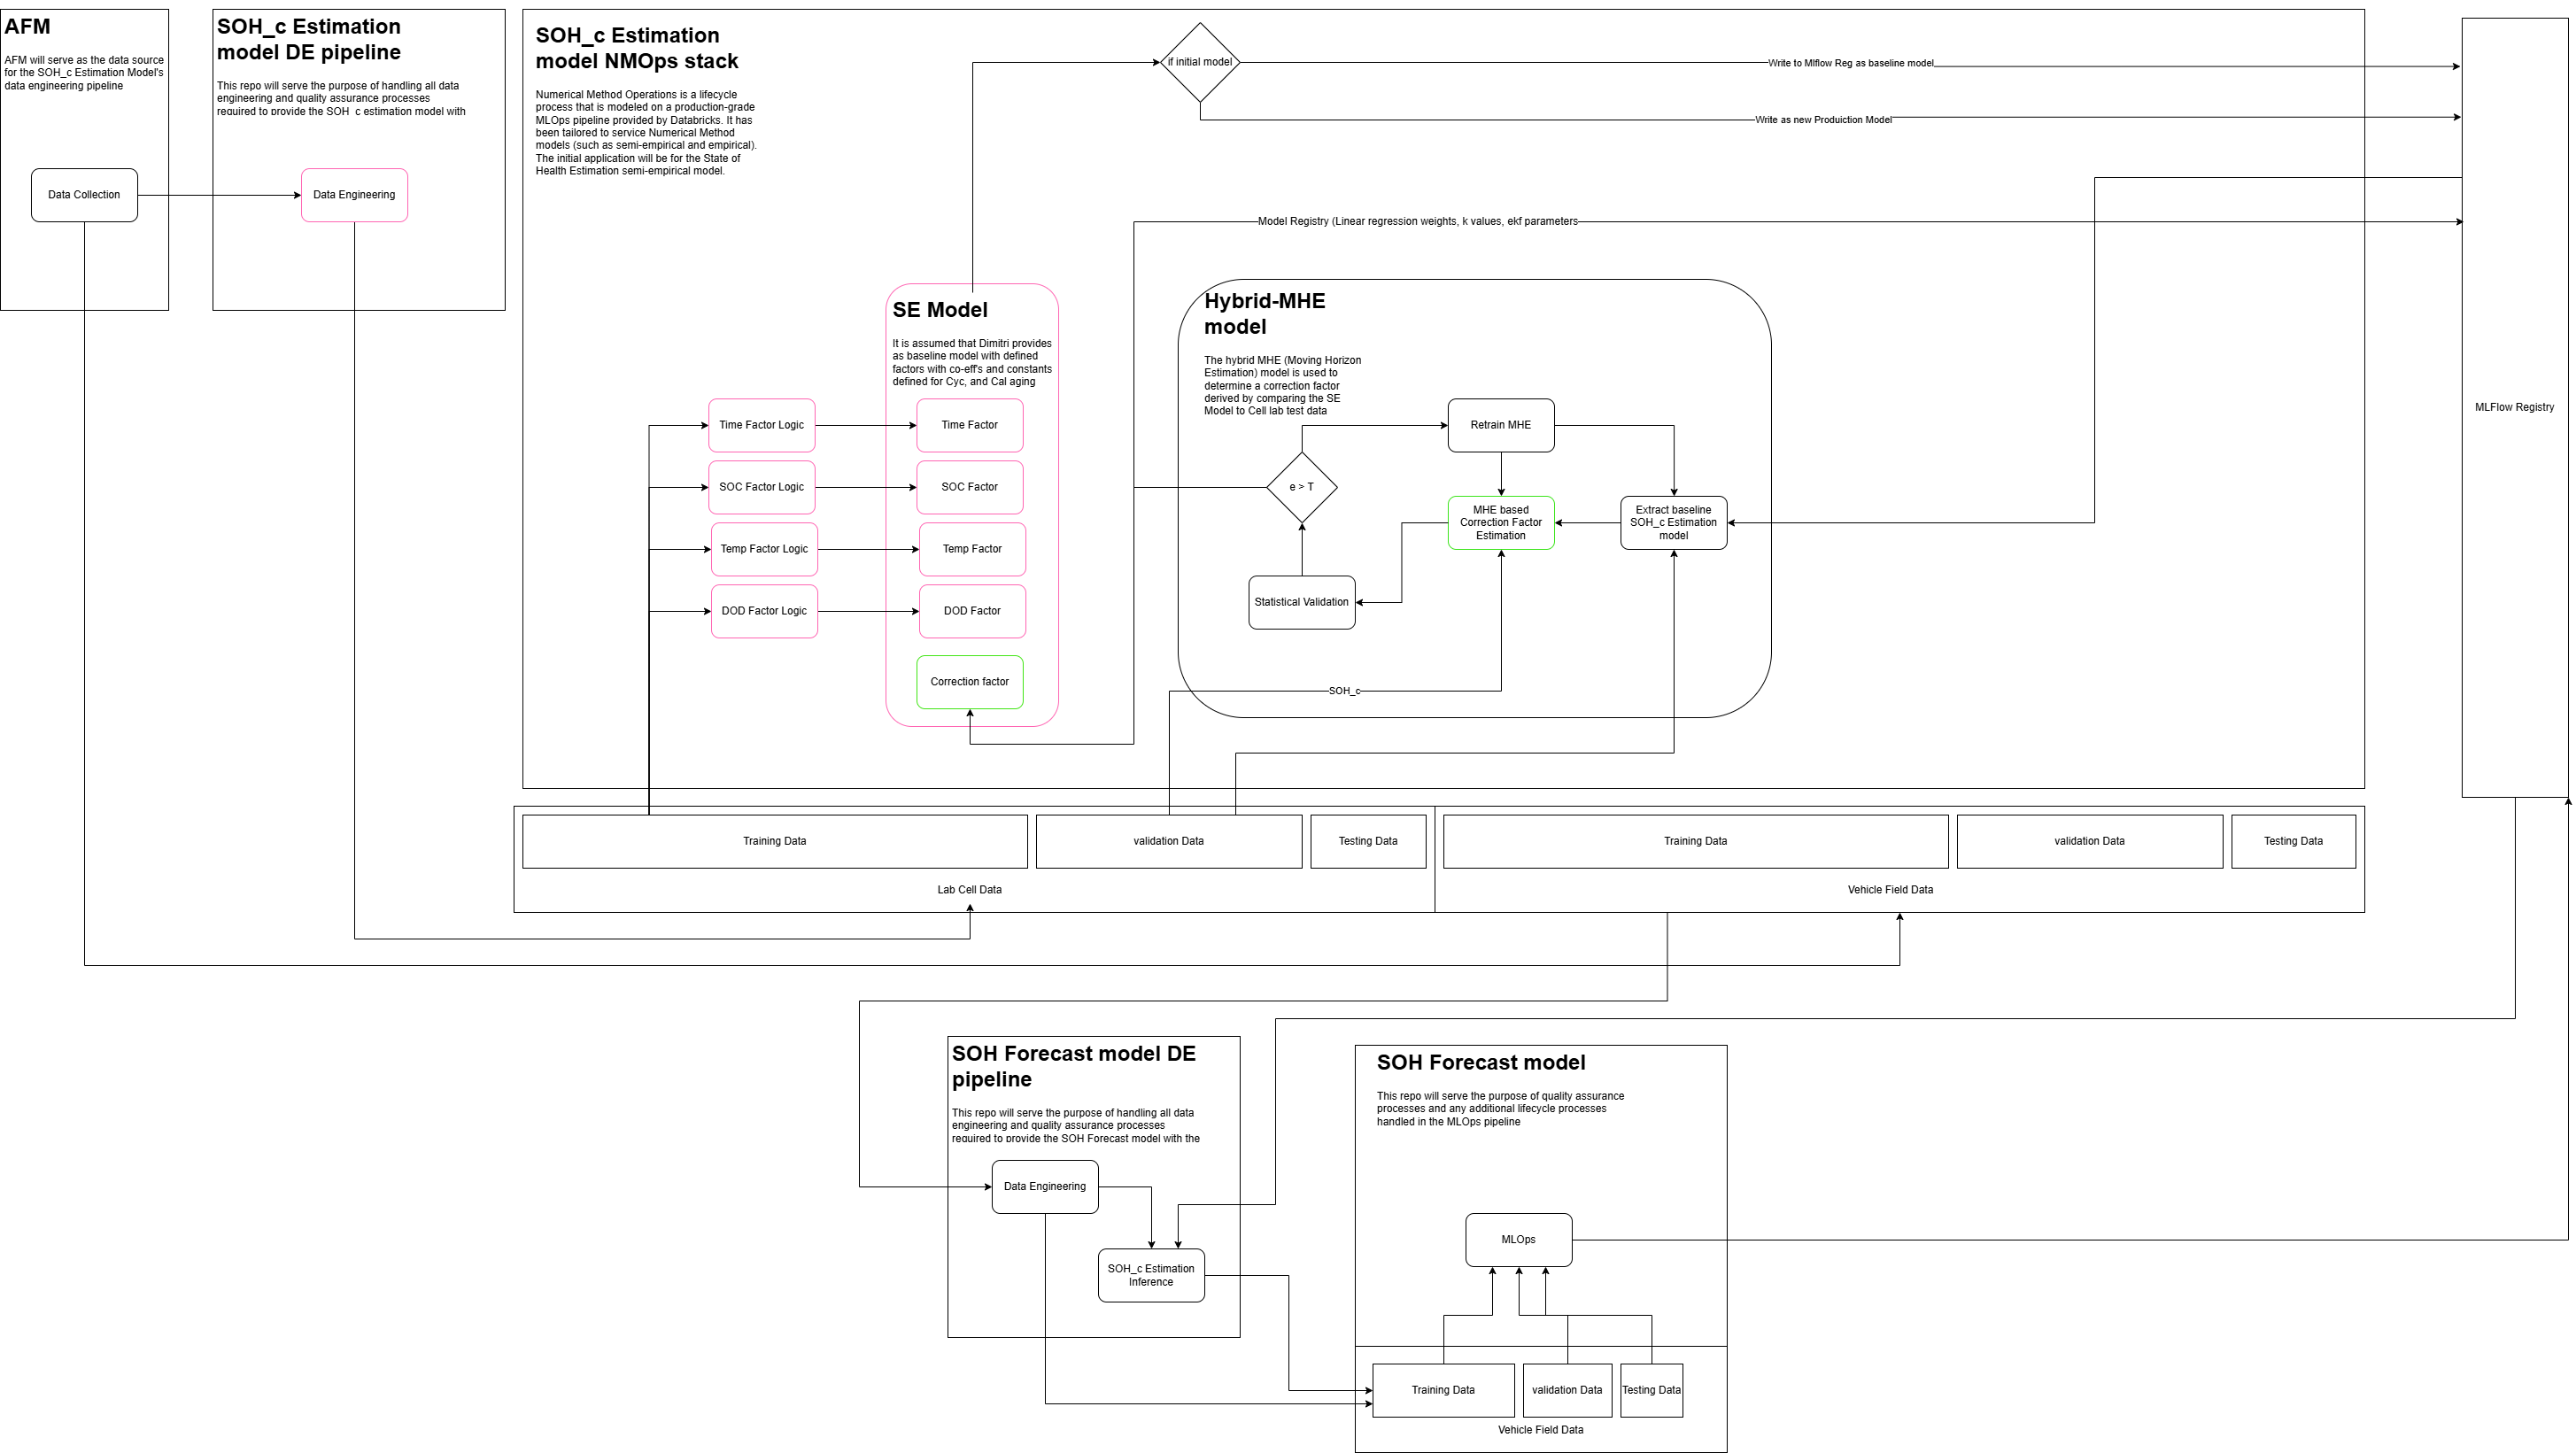
\includegraphics[width=1.0\linewidth]{thesis_template_11-11-17/NMOps-Page-1.drawio.png}
    \caption{NMOps Architecture}
    \label{fig:nmops-architecture}
\end{figure}

\section{Moving Horizon Estimation}
\label{MHE}

\subsection{Overview of Moving Horizon Estimation (MHE)}

Moving Horizon Estimation (MHE) is a deterministic optimization-based approach to dynamic state estimation that relies on a finite history of system measurements. Unlike recursive filters such as the Kalman Filter and its variants, MHE explicitly incorporates system constraints and handles model inaccuracies over a fixed time horizon. This makes it particularly suitable for nonlinear systems and applications requiring bounded estimates.

Consider the general discrete-time nonlinear system:
\begin{align}
x_{k+1} &= f(x_k, u_k) + w_k \\
y_k &= h(x_k) + v_k
\end{align}
where:
\begin{itemize}
    \item $x_k$ denotes the state vector at time step $k$,
    \item $u_k$ is the control input,
    \item $y_k$ represents the output measurement,
    \item $w_k$ and $v_k$ are process and measurement noise, respectively.
\end{itemize}

At each time step $k$, MHE solves an optimization problem over a fixed window of the $N$ most recent measurements to estimate the current state. The cost function minimizes deviations due to noise while incorporating an arrival cost from previous estimates:
\begin{align}
\min_{\{x_i, w_i\}} \quad & \ell(x_{k-N}) + \sum_{i=k-N}^{k-1} \left( \|w_i\|_{Q}^{2} + \|v_i\|_{R}^{2} \right)
\end{align}

subject to the system dynamics and measurement models:
\begin{align}
x_{i+1} &= f(x_i, u_i) + w_i, \quad i = k-N, \ldots, k-1 \\
y_i &= h(x_i) + v_i, \quad i = k-N, \ldots, k
\end{align}

where:
\begin{itemize}
    \item $\ell(x_{k-N})$ is the arrival cost, which penalizes deviation from the prior state estimate,
    \item $Q$ and $R$ are symmetric positive definite matrices weighting the process and measurement residuals,
    \item $\mathcal{X}$ and $\mathcal{W}$ denote the admissible sets for states and disturbances, respectively.
\end{itemize}

This formulation enables MHE to maintain consistency with model constraints and leverage recent measurement data for more robust and accurate state estimates. By optimizing over a horizon rather than a single step, MHE can compensate for delayed information and cope more effectively with modeling errors and transient disturbances.


The outcome of the MHE optimization problem at each time step is an updated state estimate, denoted by $\hat{x}_k$, which reflects the most likely system state given the recent window of inputs and measurements.

Conceptually, MHE is considered the estimation counterpart to Model Predictive Control (MPC). While MPC forecasts optimal control inputs over a future time horizon, MHE operates in the reverse direction—optimizing historical state estimates over a moving window of past data \cite{ZHANG2023108381}. This duality highlights MHE's backward-looking strategy, which enables it to reconstruct states more accurately by leveraging recent information.

One of MHE's key strengths lies in its ability to directly incorporate nonlinear system dynamics and explicit constraints into the estimation problem \cite{KARG2021107266}. For example, physical limitations such as enforcing a state variable to remain within the $[0, 1]$ range can be embedded as hard constraints in the optimization formulation \cite{Rao}. This flexibility gives MHE a distinct advantage over classical filters, such as the EKF, which may generate infeasible or unphysical estimates in constrained scenarios.

Furthermore, in highly nonlinear systems, MHE often delivers superior performance compared to extended Kalman filtering. This is mainly because MHE does not rely on linearization around the current estimate. Instead, it solves a nonlinear optimization problem that considers the entire horizon of measurements, resulting in more globally consistent and accurate state reconstructions \cite{Haseltine}.


While MHE offers significant benefits in flexibility, constraint handling, and nonlinear model accuracy, these advantages come with an inherent computational cost. Each estimation update involves solving an optimization problem, either linear or nonlinear, based on the most recent set of measurements \cite{Kraus}. Although solving such issues in real time may appear demanding, modern numerical solvers have made substantial progress in improving computational efficiency.

Recent implementations have shown that MHE can be executed at update rates in the range of tens of Hertz, even for moderately complex nonlinear systems with up to approximately 100 state variables \cite{Vukov}. These developments make MHE feasible for many embedded and real-time applications, particularly in fields such as battery management, where estimation fidelity is critical and computational hardware continues to evolve.

In summary, MHE delivers a robust and general framework for dynamic state estimation, capable of accommodating nonlinearities and constraints that traditional filtering methods often struggle with. The trade-off is increased computational effort, but this cost is increasingly manageable with current-generation processors and optimized solvers.


\subsection{Formal Definition and Problem Formulation of MHE}

Moving Horizon Estimation (MHE) is typically formulated for discrete-time systems. Continuous-time models, when applicable, are discretized beforehand to fit the MHE framework. The following dynamics and measurement equations describe the system:

\textbf{State Dynamics:}
\begin{equation}
    x_{k+1} = f(x_k, u_k, p) + w_k
\end{equation}

\textbf{Measurement Model:}
\begin{equation}
    y_k = h(x_k, u_k, p) + v_k
\end{equation}

Here:
\begin{itemize}
    \item $x_k \in \mathbb{R}^n$ is the system state at discrete time step $k$,
    \item $u_k$ represents the known control input or excitation,
    \item $y_k$ denotes the measured output,
    \item $f(\cdot)$ is the (possibly nonlinear) state transition function,
    \item $h(\cdot)$ defines the measurement mapping,
    \item $p$ is a vector of known or slowly varying system parameters,
    \item $w_k$ and $v_k$ denote process and measurement noise, respectively.
\end{itemize}

If applicable, physical or operational constraints can be expressed as:
\begin{equation}
    g(x_k, u_k, p) \leq 0
\end{equation}

Let $N$ denote the estimation horizon length. At time $t$, MHE uses the sequence of past measurements $y_{t-N}, \ldots, y_t$ and inputs $u_{t-N}, \ldots, u_{t-1}$ to reconstruct the most probable trajectory of system states:
\[
\{x_{t-N}, x_{t-N+1}, \ldots, x_t\}
\]

This reconstruction is typically formulated as a constrained optimization problem, minimizing a cost function that penalizes deviations from predicted model behavior and sensor observations. The problem is given by:

\begin{align}
    \min_{\{x_k, w_k, v_k\}} \quad & \frac{1}{2} \|x_{t-N} - \hat{x}_{t-N|t-N}\|_P^2 + \frac{1}{2} \sum_{k=t-N}^{t-1} \|w_k\|_{Q^{-1}}^2 + \frac{1}{2} \sum_{k=t-N}^{t} \|v_k\|_{R^{-1}}^2 \label{eq:cost_function} \\
    \text{subject to} \quad & x_{k+1} = f(x_k, u_k, p) + w_k, \quad k = t-N, \ldots, t-1 \\
    & y_k = h(x_k, u_k, p) + v_k, \quad k = t-N, \ldots, t \\
    & g(x_k, u_k, p) \leq 0, \quad k = t-N, \ldots, t
\end{align}

where:
\begin{itemize}
    \item $\hat{x}_{t-N|t-N}$ is the prior state estimate at the start of the horizon,
    \item $P$, $Q$, and $R$ are symmetric positive definite matrices representing weighting on the arrival cost, process noise, and measurement noise, respectively,
    \item The notation $\| \xi \|_M^2 = \xi^\top M \xi$ indicates the squared Mahalanobis norm weighted by $M$.
\end{itemize}

\textbf{Interpretation of Terms:}
\begin{itemize}
    \item The first term penalizes deviation from the prior knowledge of the initial state (arrival cost),
    \item The second term penalizes inconsistency with the model dynamics via process noise,
    \item The third term penalizes mismatch with actual sensor measurements.
\end{itemize}

Often, instead of estimating noise terms explicitly, $w_k$ and $v_k$ are expressed implicitly using the system equations:
\begin{align}
    w_k &= x_{k+1} - f(x_k, u_k, p) \\
    v_k &= y_k - h(x_k, u_k, p)
\end{align}

This substitution reduces the number of optimization variables and simplifies the problem to one of minimizing residual errors in dynamics and measurements.

The constraints must still be satisfied:
\[
x_{k+1} = f(x_k, u_k, p), \quad g(x_k, u_k, p) \leq 0
\]

MHE provides the ability to enforce bounds on states, outputs, or parameters throughout the estimation window—something classical filters like the Kalman filter cannot do explicitly.

At every new time step $t$, the problem is resolved with a shifted window:
\[
\{x_{t-N+1}, \ldots, x_{t+1}\}
\]
incorporating the new measurement $y_{t+1}$ and discarding the oldest data point. This shifting process maintains a fixed optimization window and ensures bounded computational complexity over time.

To express the full problem compactly using bold vectors for trajectories:
\begin{align}
    \min_{\bm{x}, \bm{w}, \bm{v}} \quad & \frac{1}{2} \|x_{t-N} - \hat{x}_{t-N|t-N}\|_P^2 + \frac{1}{2} \sum_{k=t-N}^{t-1} \|w_k\|_{Q^{-1}}^2 + \frac{1}{2} \sum_{k=t-N}^{t} \|v_k\|_{R^{-1}}^2 \\
    \text{subject to} \quad & x_{k+1} = f(x_k, u_k, p) + w_k \\
    & y_k = h(x_k, u_k, p) + v_k, \quad k = t-N, \ldots, t
\end{align}

Tuning the weighting matrices $P$, $Q$, and $R$ is essential. The arrival cost weight $P$ in particular plays a significant role in determining estimator stability and how much historical confidence is placed on the prior state.


\subsection{Assumptions and Theoretical Properties of MHE}

For Moving Horizon Estimation (MHE) to yield accurate and reliable results, certain theoretical conditions related to observability and stability must be satisfied. Specifically, the underlying system must be sufficiently observable over the moving window, and the estimation scheme must ensure bounded error as new measurements are incorporated \cite{ALESSANDRI2025112187}.

A key assumption is that the system exhibits \textit{observability}, that is, the sequence of measured outputs over the horizon must contain enough information to distinguish between different internal states. A stronger condition known as \textit{uniform observability} is required in many cases. This ensures that two distinct state trajectories result in sufficiently different output sequences over the window, as formalized through bounds involving class $\mathcal{K}$ functions \cite{Flayac_2021}.

If the horizon length $N$ is chosen to be at least as large as the system’s observability index, assuming no model mismatch or measurement noise, it is theoretically possible to reconstruct the exact state. In realistic scenarios with process and sensor noise, uniform observability guarantees that the estimation error remains bounded rather than diverging over time \cite{5718126}.

Another essential component of the MHE formulation is the \textit{arrival cost}, sometimes referred to as the prior term. Since MHE discards older measurements outside the current estimation window, the arrival cost serves to incorporate prior information and prevent estimation drift due to unmodeled past disturbances \cite{deniz2019robuststabilitymovinghorizon}. This term acts as a compact representation of all earlier information not captured within the current horizon.

If appropriately designed, the arrival cost enhances the estimator’s stability. It is often constructed to approximate either the optimal cost-to-go from a full-information estimator or the state covariance, as would be computed by a dual Kalman filter or a Riccati-based method. Theoretical guarantees show that, under conditions such as uniform observability and a properly defined arrival penalty, the estimation error of the MHE scheme remains asymptotically stable.

Two key performance guarantees that can be established under these conditions are:
\begin{itemize}
    \item Convergence of the estimated state to the true state in the ideal (noise-free) case,
    \item Bounded estimation error in the presence of bounded process and measurement noise.
\end{itemize}

In the presence of modeling errors or external disturbances, MHE can exhibit \textit{Input-to-State Stability} (ISS), where the magnitude of estimation error is bounded proportionally to the disturbance magnitude \cite{Ji}. This ensures robustness against imperfections in both the model and sensor data.

Stability analysis for MHE often relies on Lyapunov-based arguments or draws from the properties of full-information estimators. By using a sufficiently large horizon length and a well-tuned arrival cost, it is possible to bound the estimation error over time \cite{Schiller_2023}.

Even in cases where the system is not completely observable at all times, a relaxed condition known as \textit{detectability} may be sufficient. If the unobservable modes are asymptotically stable, the estimator can still maintain bounded error \cite{Schiller_2024}.

Additionally, MHE inherently provides robustness to outliers and transient sensor faults due to its batch optimization nature. The aggregated cost across multiple time steps prevents single erroneous measurements from significantly influencing the state estimate \cite{Schiller_2023}. To further improve robustness, non-quadratic penalties such as the Huber loss can be employed in the cost function, reducing sensitivity to outliers and model mismatch.

\textbf{In summary}, when system observability and model fidelity conditions are satisfied, MHE possesses strong theoretical guarantees. Specifically, it can:
\begin{itemize}
    \item Converge to the correct state trajectory as more data is accumulated,
    \item Maintain bounded error even in noisy or uncertain environments.
\end{itemize}

Achieving these properties in practical implementations requires careful design choices, especially regarding:
\begin{itemize}
    \item The estimation horizon length $N$,
    \item The structure and weight of the arrival cost term.
\end{itemize}

A horizon that is too short may behave similarly to a high-gain filter, making the estimator sensitive to noise. Conversely, increasing $N$ improves estimation accuracy at the expense of computational complexity. Hence, selecting $N$ involves balancing estimation quality against available processing resources.


\subsection{References and Example Implementations}

There is a growing body of literature and practical experimentation supporting the use of MHE in battery state estimation applications. The techniques outlined in previous sections have been validated through both academic research and early-stage industrial deployments:

\begin{itemize}
    \item \textbf{Joint State and Parameter Estimation:}  
    Several recent works extend MHE to jointly estimate system states and slowly varying parameters, such as battery capacity. In these formulations, capacity is modeled as an additional state that evolves gradually. For example, \cite{Yongzhe} presents an MHE-based method where regularization terms—functionally similar to arrival costs- are added to penalize abrupt changes in capacity unless strongly supported by the data. This enables real-time State of Health (SOH) tracking through consistent, smooth estimation of capacity fade during charge–discharge cycles.

    \item \textbf{Real-Time MHE for Embedded BMS:}  
    To enable deployment in resource-constrained embedded battery management systems (BMS), researchers have proposed computationally efficient variants of MHE. For instance, the "fast embedded MHE" method reduces complexity by using shortened horizons and partial state updates, making it suitable for low-power microcontrollers \cite{wan2024towards}. Other studies introduce multi-rate MHE architectures, exploiting that current can often be measured at higher frequencies than voltage. In such schemes, fast current-based updates are complemented by slower but more accurate voltage-based corrections, balancing accuracy and runtime efficiency.
\end{itemize}

The methods discussed here are presented generally, focusing on the underlying mathematical principles and estimation framework. These formulations are designed to be independent of specific datasets or implementation platforms. The next chapter details their practical application, including dataset characteristics, parameter selection, model tuning, and evaluation on real battery systems.


\section{Adaptive Multi-Horizon Correction Algorithm}
\label{algo}
The Adaptive Multi-Horizon Correction Algorithm is illustrated in \ref{alg:algorithm}. We will go through the steps and mathematical formulations that leverage adaptive correction factors, weighted optimization, and sequential smoothing to track SOH dynamics over battery life cycles robustly. 

\subsection{Methodology}
The Adaptive Multi-Horizon Correction Algorithm follows a sequential process consisting of:
\begin{itemize}
    \item Battery Data Processing.
    \item Adaptive window size estimation.
    \item MHE Optimization using Bayesian Search (Optuna).
    \item Weighted Averaging and stacking with Linear Regression.
    \item EKF-based smoothing and Residual Correction.
    \item Error Metrics Computation.
\end{itemize}

\subsubsection{Inputs and Outputs}
\begin{itemize}
    \item \textbf{Inputs:} \begin{itemize}
        \item \textbf{dataset\_folder:} Directory containing battery datasets.
        \item \textbf{battery\_params:} Dictionary with battery specifications.
        \item \textbf{n\_trials\_mhe:} Number of Optimization trials for MHE.
        \item \textbf{n\_trials\_ekf:} Number of Optimization trials for EKF.
    \end{itemize}
    \item \textbf{Outputs:} \begin{itemize}
        \item \textbf{all\_results:} Dictionary storing optional parameters, SOH predictions, and error metrics for each battery.
    \end{itemize}
\end{itemize}

\subsubsection{Battery Preprocessing}
Each battery dataset is first processed to extract:
\begin{itemize}
    \item \textbf{Final\_cyclic\_aging:} SOH estimate from the Semi-Empirical model.
    \item \textbf{Ground\_truth\_soh:} SOH from the test bench data.
\end{itemize}
Final cyclic aging is rescaled to match the mean of the ground truth:
\begin{equation}
    \text{Final\_cyclic\_aging\_scaled} = \text{Final\_cyclic\_aging} \times \frac{\mu_{\text{fa}}}{\mu_{\text{gt}}}
\end{equation}
Where:
\begin{itemize}
    \item $\mu_{\text{gt}}$ is the mean of the ground truth sequence,
    \item $\mu_{\text{fa}}$ is the mean of the final cyclic aging sequence.
\end{itemize}

\subsubsection{Adaptive Window Size Computation}
To handle varying degradation rates, window sizes are adapted based on SOH changes:
\begin{enumerate}
    \item Computer first differences: \begin{equation}
    \Delta \text{SOH}_i = \left| \text{SOH}_{i+1} - \text{SOH}_i \right|\end{equation}
    \item Define a threshold $\tau$ as the 75th percentile of the set of first differences $\Delta \text{SOH}$.
    \item Assign window sizes according to:
\begin{equation}
\text{window\_size}_i = 
\begin{cases}
3, & \text{if } \Delta \text{SOH}_i > \tau \\
10, & \text{otherwise}
\end{cases}
\end{equation}
\end{enumerate}

\subsubsection{Moving Horizon Estimation (MHE)}
For each unique window size, the MHE problem is formulated as a minimization of a hybrid objective function involving:
\begin{itemize}
    \item \textbf{Huber Loss} for robust error handling: \begin{equation}
L_\delta(r) = 
\begin{cases}
\frac{1}{2} r^2, & \text{if } |r| \leq \delta \\
\delta (|r| - \frac{1}{2} \delta), & \text{otherwise}
\end{cases}
\end{equation}
where:
\begin{itemize}
    \item \( r \) is the residual between the corrected State of Health (SOH) and the ground truth,
    \item \( \delta = 1.0 \) is the threshold parameter.
\end{itemize}
\item Define the penalty term \( k_{\text{penalty}} \) as:
\begin{equation}
k_{\text{penalty}} = 
\begin{cases}
1000 \times \left( |k - k_{\text{prev}}| - 0.1 \right), & \text{if } |k - k_{\text{prev}}| > 0.1 \\
0, & \text{otherwise}
\end{cases}
\end{equation}
Where:
\begin{itemize}
    \item \( k \) is the current correction factor,
    \item \( k_{\text{prev}} \) is the previous correction factor.
\end{itemize}
\item Define the L2 regularization penalty as:
\begin{equation}
L2_{\text{penalty}} = 0.01 \times k^2
\end{equation}
where:
\begin{itemize}
    \item \( k \) is the correction factor or model parameter being regularized.
\end{itemize}
\item Define the penalty based on the Mean Squared Error (MSE) as:
\begin{equation}
\text{penalty} = 
\begin{cases}
1000 \times | \text{MSE} - 17 |, & \text{if } \text{MSE} < 9 \text{ or } \text{MSE} > 25 \\
0, & \text{otherwise}
\end{cases}
\end{equation}
Where:
\begin{itemize}
    \item MSE is the Mean Squared Error between predicted and ground truth values.
\end{itemize}
\end{itemize}
Thus, the Moving Horizon Estimation (MHE) optimization objective is defined as:
\begin{equation}
\text{Objective} = \text{Huber Loss} + k_{\text{penalty}} + L2_{\text{penalty}} + \text{penalty}
\end{equation}
Where:
\begin{itemize}
    \item \textbf{Huber Loss} penalizes residual errors between the corrected SOH and ground truth,
    \item \( k_{\text{penalty}} \) penalizes large deviations in the correction factor \(k\),
    \item \( L2_{\text{penalty}} \) provides regularization to keep \(k\) small,
    \item \textbf{penalty} enforces the MSE to remain within the desired range \([9, 25]\).
\end{itemize}

Bayesian optimization, implemented via the Optuna framework \cite{akiba2019optunanextgenerationhyperparameteroptimization}, is employed to find the global optimum.

\subsubsection{Weighted Averaging of MHE Solutions}
After solving individual MHE problems, a weighted aggregation is performed to compute the corrected SOH as:
\begin{equation}
\text{Corrected\_SOH} = \sum_i \left( \frac{w_i}{\sum_j w_j} \times k_i \times \text{Final\_cyclic\_aging\_scaled} \right)
\end{equation}
Where:
\begin{itemize}
    \item \( w_i = \frac{1}{\text{loss}_i} \) is the weight assigned to the \(i\)-th MHE solution, inversely proportional to its associated loss,
    \item \( k_i \) is the correction factor from the \(i\)-th MHE,
    \item \text{Final\_cyclic\_aging\_scaled} is the scaled cyclic aging sequence.
\end{itemize}

\subsubsection{Stacking Model: Linear Regression}
A simple stacked regression model is trained as:
\begin{equation}
\text{Stacked\_SOH} =\\ \alpha \times \text{Final\_cyclic\_aging\_scaled} + \beta \times \text{Local\_Corrected\_SOH} + \gamma
\end{equation}
where:
\begin{itemize}
    \item \( \alpha, \beta, \gamma \) are coefficients learned by minimizing the least squares error.
\end{itemize}

\subsubsection{EKF Smoothing}
Using the following equations, an Extended Kalman Filter (EKF) is applied to reduce sequential noise.

State Prediction:

\begin{align}
x_{k|k-1} &= x_{k-1} + \text{trend\_rate} \\
P_{k|k-1} &= P_{k-1} + Q
\end{align}

Measurement Update:

\begin{align}
K_k &= \frac{P_{k|k-1}}{P_{k|k-1} + R} \\
x_k &= x_{k|k-1} + K_k (z_k - x_{k|k-1}) \\
P_k &= (1 - K_k) P_{k|k-1}
\end{align}

Where:
\begin{itemize}
    \item \( Q \) and \( R \) represent the process and measurement noise covariances, respectively,
    \item \( \text{trend\_rate} \) is a drift term accounting for expected gradual changes in the state.
\end{itemize}

Hyperparameter Optimization:

The hyperparameters \( Q \), \( R \), and \( \text{trend\_rate} \) are optimized via Bayesian optimization using the Optuna framework \cite{akiba2019optunanextgenerationhyperparameteroptimization}, to minimize the post-smoothing Huber loss.

\subsubsection{Error Metrics}
The final evaluation metrics include:

Mean Squared Error (MSE):

\begin{equation}
\text{MSE} = \frac{1}{N} \sum_{i=1}^{N} (y_i - \hat{y}_i)^2
\end{equation}

Root Mean Squared Error (RMSE):

\begin{equation}
\text{RMSE} = \sqrt{\text{MSE}}
\end{equation}

Both metrics are computed against the ground truth and the scaled cyclic aging baselines.


\begin{algorithm}
\caption{Battery SOH Estimation with MHE, Stacking, and EKF}
\label{alg:algorithm}
\begin{algorithmic}[1]
\ENSURE all\_results (dictionary)

\STATE Load battery parameters from \texttt{battery\_params.json} into \texttt{params}
\STATE Initialize \texttt{all\_results = \{\}}

\FOR{each \texttt{battery\_name} in \texttt{params}}
    \STATE \texttt{macro\_df = process\_battery(battery\_name, dataset\_folder)}
    \STATE Scale \texttt{Final\_cyclic\_aging}:
    \STATE \hspace{0.5cm} \texttt{scaling\_factor = mean(ground\\\_truth\_soh) / mean(Final\_cyclic\_aging)}
    \STATE \hspace{0.5cm} \texttt{Final\_cyclic\_aging\_scaled = Final\_cyclic\_aging} $\times$ \texttt{scaling\_factor}

    \STATE Compute adaptive \texttt{window\_sizes} based on 75th percentile of $\Delta$SOH.

    \STATE Initialize \texttt{mhe\_results = [ ]}, \texttt{prev\_k = None}

    \FOR{each unique \texttt{window\_size} in \texttt{window\_sizes}}
        \STATE Initialize Optuna study (TPE Sampler, startup trials=20)
        \FOR{each trial (n\_trials\_mhe // number of unique window sizes)}
            \STATE Suggest \texttt{window\_size} and \texttt{global\_k}
            \STATE Compute objective combining Huber Loss, k\_penalty, L2\_penalty, and MSE penalties
        \ENDFOR
        \STATE Store best (\texttt{window\_size}, \texttt{global\_k}, \texttt{loss}) in \texttt{mhe\_results}
        \STATE Update \texttt{prev\_k}
    \ENDFOR

    \STATE Perform weighted averaging of MHE results to compute \texttt{Local\_Corrected\_SOH}

    \STATE Apply stacking (Linear Regression) to predict \texttt{Stacked\_SOH} from \texttt{Final\_cyclic\_aging\_scaled} and \texttt{Local\_Corrected\_SOH}

    \STATE Apply EKF smoothing:
    \STATE \hspace{0.5cm} Initialize Optuna study (startup trials=10)
    \STATE \hspace{0.5cm} Optimize (Q, R, trend\_rate)
    \STATE \hspace{0.5cm} Run EKF to compute \texttt{Smoothed\_SOH}

    \STATE Compute error metrics: MSE, RMSE against ground truth and final cyclic aging.

    \STATE Save \texttt{macro\_df} to file and update \texttt{all\_results[battery\_name]} with results.

    \STATE Print optimization values and plot SOH curves.
\ENDFOR

\RETURN \texttt{all\_results}

\end{algorithmic}
\end{algorithm}

\subsection{Example}
This section illustrates the application of optimized correction factors ($k$ values) to battery degradation data. Using a simple 10-cycle example, we demonstrate how correction factors, optimized by Moving Horizon Estimation (MHE), are blended through weighted averaging to enhance State of Health (SOH) prediction.

\textbf{Problem Setup}

We consider a battery named \texttt{B0005} with data for 10 cycles:

\begin{itemize}
    \item \textbf{Cycle indices}: $[0, 1, 2, 3, 4, 5, 6, 7, 8, 9]$
    \item \textbf{Final\_cyclic\_aging\_scaled} (\%): $[80, 79, 78, 77, 76, 75, 74, 73, 72, 71]$
    \item \textbf{Ground truth SOH} (\%): $[81, 80, 79, 78, 77, 76, 75, 74, 73, 72]$
\end{itemize}

The goal is to correct the \texttt{Final\_cyclic\_aging\_scaled} series so it closely matches the ground truth SOH.

Two window sizes were selected based on SOH change dynamics:
\begin{itemize}
    \item Window size 3 (sensitive to short-term changes)
    \item Window size 10 (captures global trends)
\end{itemize}

The optimized correction factors obtained via MHE are:
\[
k_1 = 1.0125 \quad (\text{for window size 3}), \qquad k_2 = 1.0140 \quad (\text{for window size 10})
\]
The associated optimization losses are:
\[
\text{Loss}_1 = 10, \quad \text{Loss}_2 = 12
\]

\textbf{Correction Process}

\textbf{Applying $k_1$ for Window Size 3}

The 10 cycles are partitioned into windows of size 3:

\[
[0,1,2],\quad [3,4,5],\quad [6,7,8],\quad [9]
\]

Applying $k_1$ to each chunk:

\begin{align*}
\text{Chunk [0-2]} &: [80, 79, 78] \times 1.0125 = [81.000, 79.9875, 78.975]\\
\text{Chunk [3-5]} &: [77, 76, 75] \times 1.0125 = [77.9625, 76.9500, 75.9375]\\
\text{Chunk [6-8]} &: [74, 73, 72] \times 1.0125 = [74.925, 73.9125, 72.900]\\
\text{Chunk [9]}   &: [71] \times 1.0125 = [71.8875]
\end{align*}

Thus, the whole corrected series for window size 3 is:

\[
\text{SOH}_3 = [81.000, 79.9875, 78.975, 77.9625, 76.950, 75.9375, 74.925, 73.9125, 72.900, 71.8875]
\]

\textbf{Applying $k_2$ for Window Size 10}

For window size 10, the entire dataset is treated as a single window:

\[
[0,1,2,3,4,5,6,7,8,9]
\]

Applying $k_2$:

\begin{align*}
\text{SOH}_{10} = &[80 \times 1.0140, 79 \times 1.0140, 78 \times 1.0140, 77 \times 1.0140,\\
&76 \times 1.0140, 75 \times 1.0140, 74 \times 1.0140, 73 \times 1.0140, 72 \times 1.0140, 71 \times 1.0140] \\
= &[81.120, 80.106, 79.092, 78.078, 77.064, 76.050, 75.036, 74.022, 73.008, 71.994]
\end{align*}

\textbf{Computing Weights for Blending}

The weights are computed as the inverse of the optimization losses:

\[
\text{Weight}_1 = \frac{1}{10} = 0.1, \quad \text{Weight}_2 = \frac{1}{12} \approx 0.08333
\]
Total weight:
\[
\text{Total Weight} = 0.1 + 0.08333 = 0.18333
\]
Normalized weights:
\[
\text{Normalized Weight}_1 = \frac{0.1}{0.18333} \approx 0.54545, \quad \text{Normalized Weight}_2 = \frac{0.08333}{0.18333} \approx 0.45455
\]

\textbf{Blending the Corrected SOHs}

The final corrected SOH at each cycle is computed by weighted averaging:

\[
\text{Final SOH}_i = (0.54545 \times \text{SOH}_3[i]) + (0.45455 \times \text{SOH}_{10}[i])
\]

Example calculations:

\begin{align*}
\text{Cycle 0}: \quad &81.0545 = (0.54545 \times 81.000) + (0.45455 \times 81.120)\\
\text{Cycle 1}: \quad &80.0402 = (0.54545 \times 79.9875) + (0.45455 \times 80.106)\\
\text{Cycle 2}: \quad &79.0260 = (0.54545 \times 78.975) + (0.45455 \times 79.092)\\
\end{align*}

Following the same blending process for all cycles yields:

\[
\text{Local\_Corrected\_SOH} \approx [81.0545, 80.0402, 79.0260, 77.9977, 76.9834,~75.9692,~74.9550,....]
\]

This example illustrates how multiple MHE-optimized correction factors ($k_1$ and $k_2$) are applied to different window sizes and blended to produce a robust SOH trajectory. The final SOH curve benefits from local sensitivity and global consistency by giving more weight to correction factors with lower losses.
